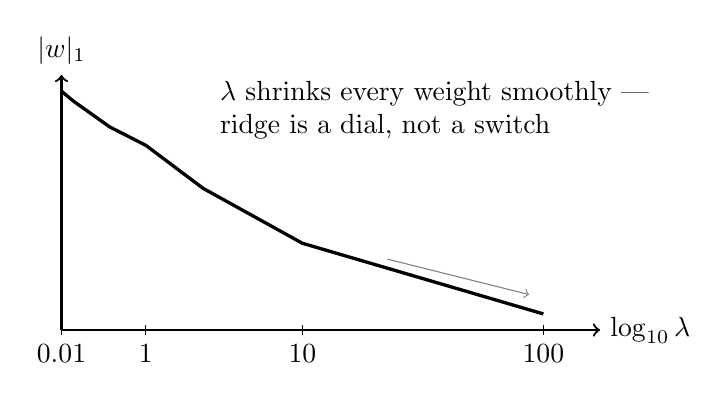
\begin{tikzpicture}[scale=0.9]
\draw[->, thick] (0,0) -- (7.6,0) node[right] {$\log_{10}\lambda$};
\draw[->, thick] (0,0) -- (0,3.6) node[above] {$|w|_1$};
% real numbers: lam .01 .1 .5 1 3 10 100 -> |w|1 9.36 8.97 7.96 7.24 5.55 3.40 .63
% x = (log10 lam + 2)*1.7 ; y = |w|1*0.36
\draw[very thick] plot coordinates {
  (0,3.370) (0.17,3.229) (0.68,2.866) (1.19,2.606)
  (2.00,1.998) (3.40,1.224) (6.80,0.227)};
\foreach \x/\lam/\v in {0/{0.01}/{9.36}, 1.19/{1}/{7.24},
  3.40/{10}/{3.40}, 6.80/{100}/{0.63}}{
  \draw (\x,0.07) -- (\x,-0.07) node[below] {$\lam$};}
\node[align=left, anchor=west] at (2.1,3.1) {$\lambda$ shrinks every
  weight smoothly ---\\ ridge is a dial, not a switch};
\draw[->, gray] (4.6,1.0) -- (6.6,0.5);
\end{tikzpicture}
